\section{Prototipo}
La arquitectura que se propone en este trabajo, como ya se mencion\'o antes cuenta con tres capas: recuperaci\'on de datos, gesti\'on de contexto, y uso de contexto. Para poder acoplar la arquitectura primero se tiene que dar de alta un modelo del groupware. Para esto se cre\'o una plataforma para registrar casos de estudio en la que se establece el nombre del caso de estudio y todos sus elementos, una vez creado el meta modelo del groupware se instancia el modelo de dominio del Groupware y se administran las interacciones para poder relacionar sus elementos, ya con este modelo se pueden capturar la informaci\'on contextual que el sistema va a enviar a la arquitectura. 

\begin{figure}[h!]
\centering
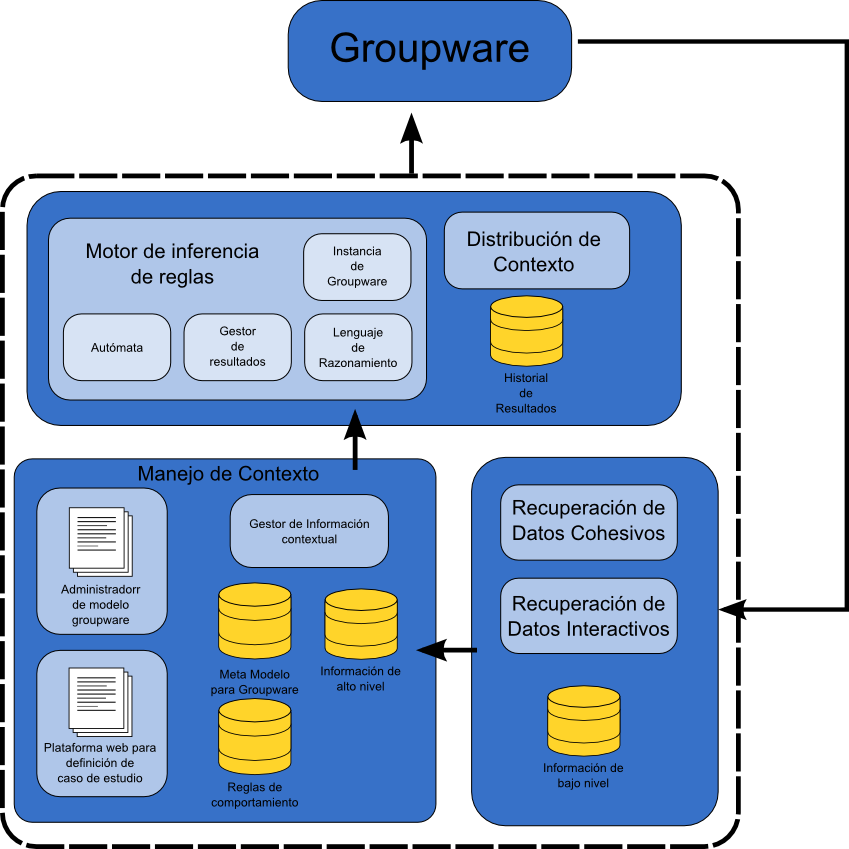
\includegraphics[scale=0.40]{images/arqui2}
\caption{Arquitectura propuesta}
\label{ARCH:propuesta}
\end{figure}

La arquitectura se divide en tres capas; la capa de recuperaci\'on de datos, la capa de gestion de datos y la capa de uso de contexto. En la primera capa, la de recuperac\'on de datos, se captura informaci\'on contextual enviada por el groupware por medio de servicios web din\'amicos, publicados para la comunicaci\'on entre la arquitectura y el sistema, estos datos son enviados en un formato espec\'ifico, en este caso serializados en Json. Seguido de este m\'odulo est\'a el de gesti\'on contextual, este gestor se encarga de registrar, actualizar y recuperar la informaci\'on contextual en bases de datos, es a este nivel donde se define el meta modelo y  se instancia el modelo de dominio del sistema y donde los datos enviados desde el groupware se registran, desde ahí son recuperados para inferir resultados en niveles superiores. Cabe mencionar que en esta plataforma tambi\'en se definen las reglas de comportamiento para el groupware. En estas reglas se definen los resultados que debe de arrojar el motor de inferencia basado en eventos del sistema, estos eventos se describen como interacciones, una interacci\'on $I$ esta compuesta b\'asicamente de un $Actor$ y una $Tarea$(\textit{e.g.} \textbf{Jugador se mueve}), a partir de este tipo de interaci\'on surgen otras, entre las que se identifican est\'an la interacci\'on en la que se afecta a otra entidad como un actor o conjunto de actores $A$ u objeto o conjunto de objetos $O$; y la interacci\'on en la que un actor $A$ realiza una tarea con ayuda de un objeto $O$. Adem\'as de las interacciones tambi\'en se da el caso en el que se necesiten comparar valores de los atributos de  los elementos, para esto se definieron las expresiones compuestas por un elemento del modelo de dominio, un atributo del elemento, un operador que compara el atributo con un valor v\'alido definido en el meta modelo, entre los operadores de comparaci\'on se encuentran '=', '\textless', '\textgreater', '$\neg$'(\textit{i.e.} de igualdad, mayor que, menor que, y diferencia).

En esta capa se encuentra una plataforma en la que se pueden dar de alta elementos del modelo de actividad. Para poder ingresar al sistema con un caso de estudio, se tiene que dar de alta con un nombre y una contrase\~na para el logueo, esto se lleva a cabo en la vista mostrada en la figura \ref{Ptf:registro1}

\begin{figure}
\centering
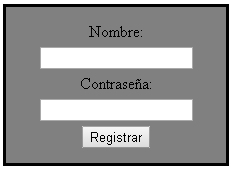
\includegraphics[scale=.8]{images/RegistroProto.png}
\caption{Registro de caso de estudio}
\label{Ptf:registro1}
\end{figure}

En la figura \ref{Ptf:login} se observa un formulario para le logueo al sistema, esto para poder asociar los elementos a un caso de estudio en espec\'ifico y los elementos est\'en disponibles s\'olo para los casos para los que fueron especificados.
\newpage
\begin{figure}[h!]
\centering
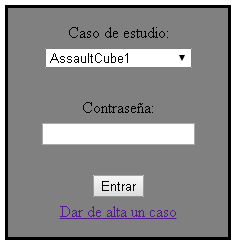
\includegraphics[scale=.7]{images/LoginProto.png}
\caption{Login de acceso a la plataforma.}
\label{Ptf:login}
\end{figure}

Una  vez dentro de la plataforma, en la pantalla principal mostrada en la figura\ref{Ptf:home} se encuentran pesta\~nas que dan acceso a las vistas de defnici\'on de los elementos del meta modelo y la pantalla para la definici\'on de reglas. Los elementos se encuentran divididos en elementos cohesivos e interactivos.

\begin{figure}[h!]
\centering
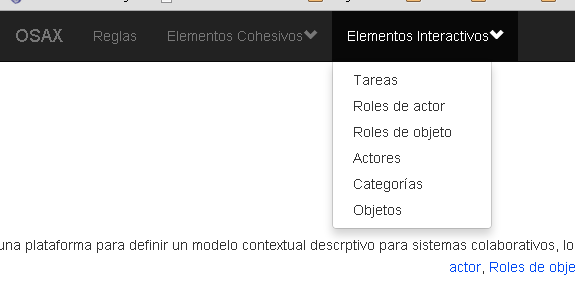
\includegraphics[scale=.7]{images/homeProto.png}
\caption{P\'agina inicial de la plataforma}
\label{Ptf:home}
\end{figure}

Al acceder a una vista de definici\'on de elemento, aparece un formulario similar a  la figura \ref{Ptf:registro} en la que se define el n\'umero de atributos, adicionales a los presentados, que van a formar parte del elemento del dominio del groupware y el valor que van a tomar, despu\'es de definir los atributos del elemento, se registra para que sea accesible por los elementos que puedan hacer uso de ellos.
\newpage

\begin{figure}[h!]
\centering
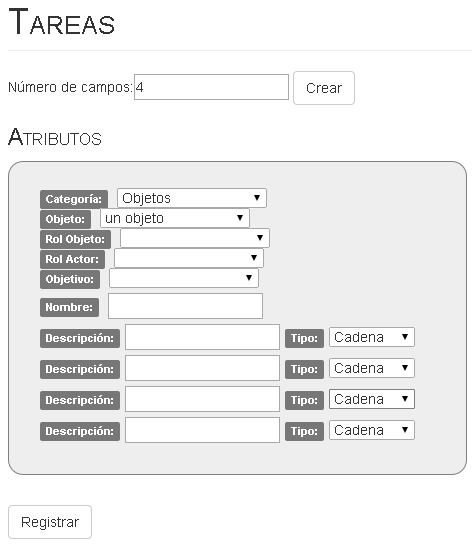
\includegraphics[scale=.6]{images/TareasProto.png}
\caption{Vista de registro de elementos}
\label{Ptf:registro}
\end{figure}

En la \'ultima capa de la arquitectura, uso de contexto, la informaci\'on es procesada por un motor de inferencia que trabaja con interacciones enviadas desde el groupware y  que da como resultado otra interacci\'on o conjunto de interacciones que representan una acci\'on propia del groupware que puede concluir en la presentaci\'on de informaci\'on al usuario que lo necesite o la ejecuci\'on de un comando para adaptar el groupware a la situaci\'on actual del usuario. Dentro del motor de inferencia se llevar\'a un registro de las instancias de las interacciones que se llevan a cabo en el groupware, as\'i se puede comparar su estado actual con las reglas de comportamiento definidas para ofrecer resultados coherentes en tiempo real. Los resultados obtenidos son gestionados por un administrador de resultados que almacena los datos para mantener registro hist\'orico del comportamiento del groupware. Una vez obtenidos y almacenados los resultados un m\'odulo de distribuci\'on se encarga de enviar las interacciones al groupware con la informaci\'on necesaria. Este proceso es iterativo, ya que funciona por el tiempo en el que el groupware opera.

\section{Conclusiones}
Esta arquitectura está diseñada para apoyar el trabajo colaborativo, pero su modelo se puede utlizar para brindar consciencia contexual a otro tipo de sistemas, se implementar\'a en el groupware Assault Cube y se probar\'an sus resultados, con esto se pretende evaluar el desempe\~no de la arquitectura. Har\'ia falta una interfaz acoplable al groupware para que este se pudiera comunicar con la arqutiectura con facilidad. La eficiencia de los resultados depende de las reglas definidas, si las reglas est\'an establecidas para apoyar al grupo de trabjo colaborativo entonces la arquitectura tambi\'en.
 